A strong correlation between observed and expected \ddg\ was not found for any of the structures nor for the set of mutations taken as a whole.
Despite this single side chain conformations were in very good agreement between predicted side chain locations and crystal structures, suggesting that sufficient sampling was done in the side chain prediction step.

%%%%%%%%%%%%%%%%%%%%%%%%%%%%%%%%%%%%%%%%%%%%%%%%%%%%%%%%%%%%%%%%%%%%%%%%%%%%%%%%%%%%%%%%%%%%%%%%%%%%
%1BRSa
\FloatBarrier
\subsection{Barstar-Barnase Complex (Barnase Mutated)}
The first complex examined is the Barstar-Barnase complex.
This complex is frequently used as a case study in protein-protein interaction, as the complex exhibits one of the highest known binding affinities, K\subscript{d} = 0.01 pM \cite{hartley1988barnase,hartley1989barnase,schreiber1993interaction}.
Experimental affinity data is available from alanine scanning mutations for eight residues in barnase and six residues for barstar.
Mutations to each chain were considered independently, and mutations to barstar are covered in the following section.
The correlation between predicted and experimental \ddg\ binding was not significant, see figure \ref{figure:computational_mutation_scanning/1BRSa_ddg}, $R^{2}=0.08$.

\begin{figure}[h]
    \centering
    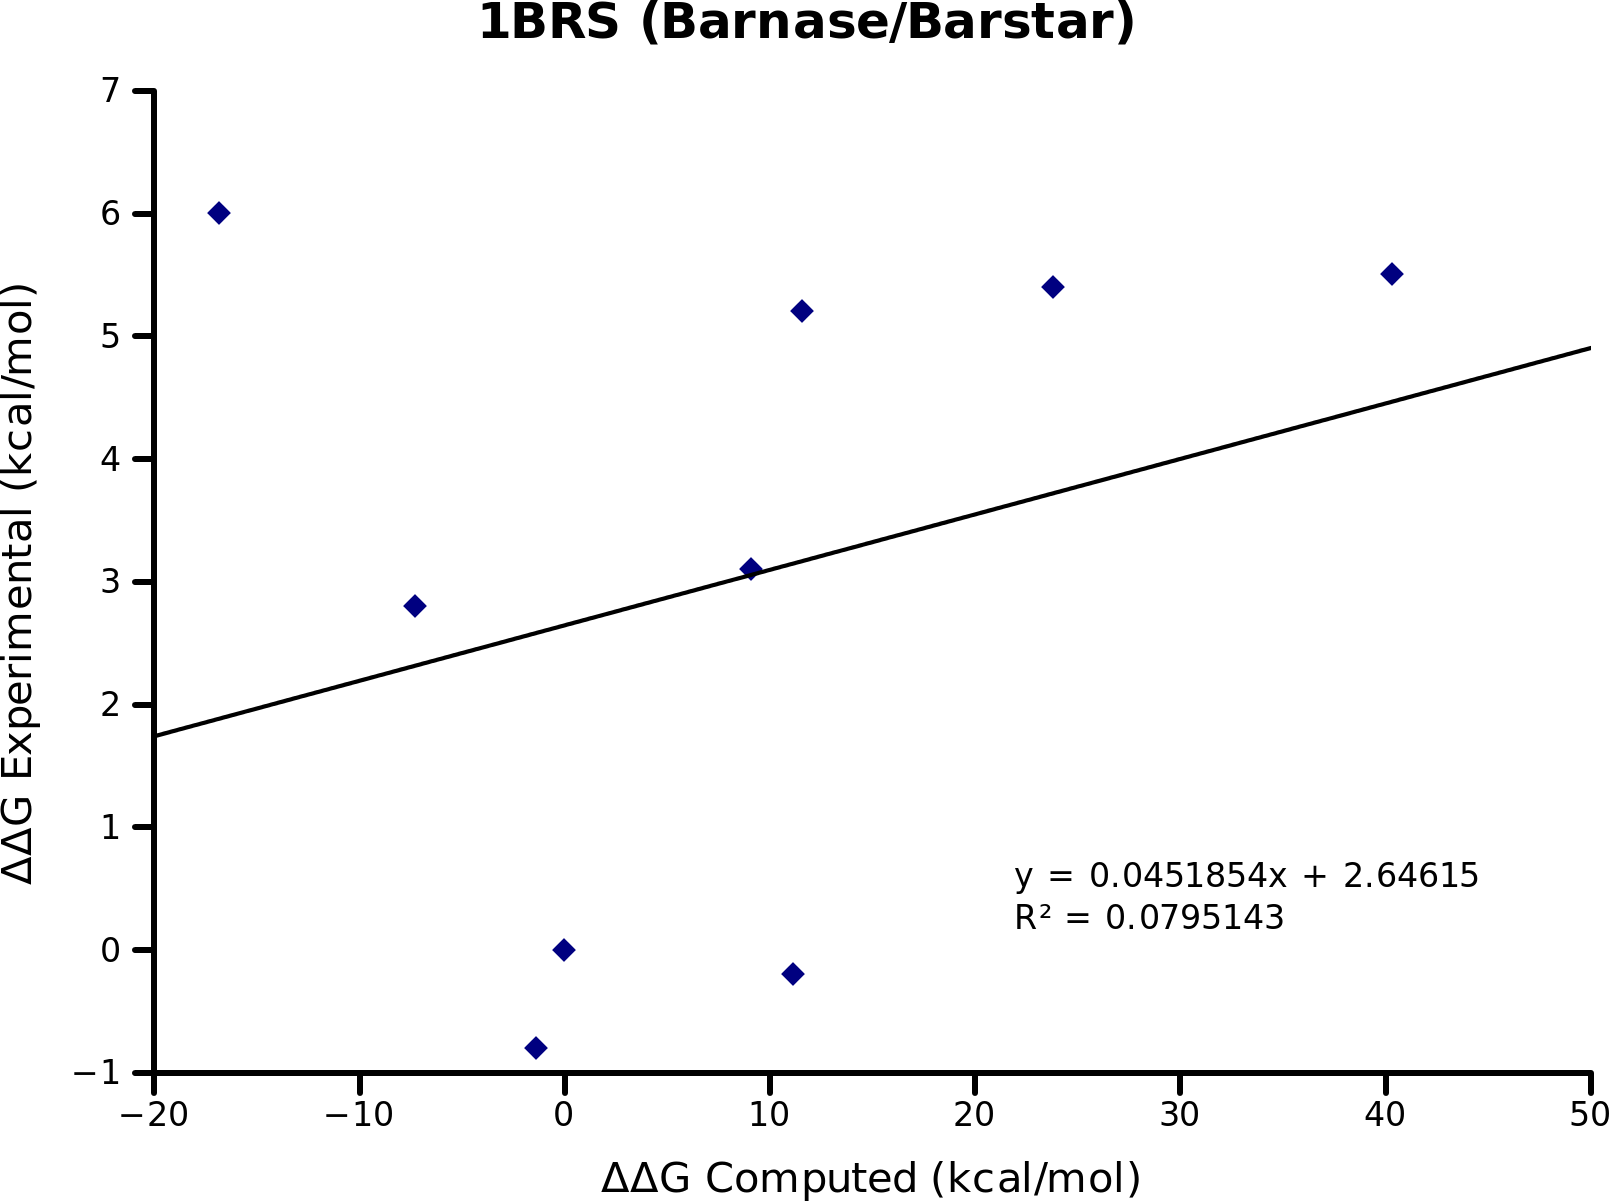
\includegraphics[width=0.65\textwidth]{figures/1brs_barnase_barstar.png}
    \caption{Computed versus experimental \ddg\ binding for 8 alanine mutations in the Barstar-Barnase binding pair.
    Crystal structure used for computations was 1BRS.
    Specific amino acids mutated were residues 27, 54, 58, 59, 60, 73, 87, and 102, all of chain A.
    Experimental binding affinity taken from \protect\cite{thorn2001asedb}.}
    \label{figure:computational_mutation_scanning/1BRSa_ddg}
\end{figure}

Table \ref{table:1BRSa_results} shows the computed and experimental \ddg's used to generate figure \ref{figure:computational_mutation_scanning/1BRSa_ddg}.
\begin{table}[H]
\centering
\label{table:1brs_a_results}
\begin{tabular}{|c|c|c|}
\hline
Residue & \ddg\ calculated & \ddg\ experimental \\
\hline
native & 0 & 0 \\
27 & 23.82 & 5.4 \\
54 & -1.37 & -0.8 \\
58 & 9.09 & 3.1 \\
59 & 11.58 & 5.2 \\
60 & 11.15 & -0.2 \\
73 & -7.28 & 2.8 \\
87 & 40.32 & 5.5 \\
102 & -16.83 & 6 \\
\hline
\end{tabular}
\caption{}
\end{table}

Table \ref{table:1BRSa_rmsd} shows the root mean square distance for the side chain conformations predicted during the mutation scan to the crystal structure.
All eight side chains are predicted within 1.3 angstroms of the native structure, and the median prediction is 0.359 angstroms, which is a very accurate prediction and generally sufficiently accurate to reproduce native binding interactions.
\begin{table}[h]
\centering
\begin{tabular}{|c|c|c|}
\hline
Residue & Amino Acid & RMSD \\
\hline
A:27 & LYS & 1.213 \\
A:54 & ASP & 0.920 \\
A:58 & ASN & 0.121 \\
A:59 & ARG & 0.421 \\
A:60 & GLU & 0.138 \\
A:73 & GLU & 0.994 \\
A:87 & ARG & 0.297 \\
A:102 & HIS & 0.276 \\
\hline
\end{tabular}
\caption{RMSD of mutated side chains in barnase, in a barnase-barstar complex (chain A of PDBid 1BRS), during the mutation scanning experiments.}
\label{table:1BRSa_rmsd}
\end{table}


Despite the lack of correlation of predicted binding affinities with experimental values, single single side chain conformations predicted in the course of the mutation scan were in very good agreement with crystal structures.
This indicates that sufficient sampling was done in the side chain prediction step of the computation.
Figure \ref{figure:computational_mutation_scanning/1brs_a_58} shows the predicted and crystal conformations for Asp 58 of barnase.
The conformations are almost identical, differing by only 0.121 angstroms, or less than the resolution of the crystal structure (2.0 angstroms).
\begin{figure}[h]
    \centering
    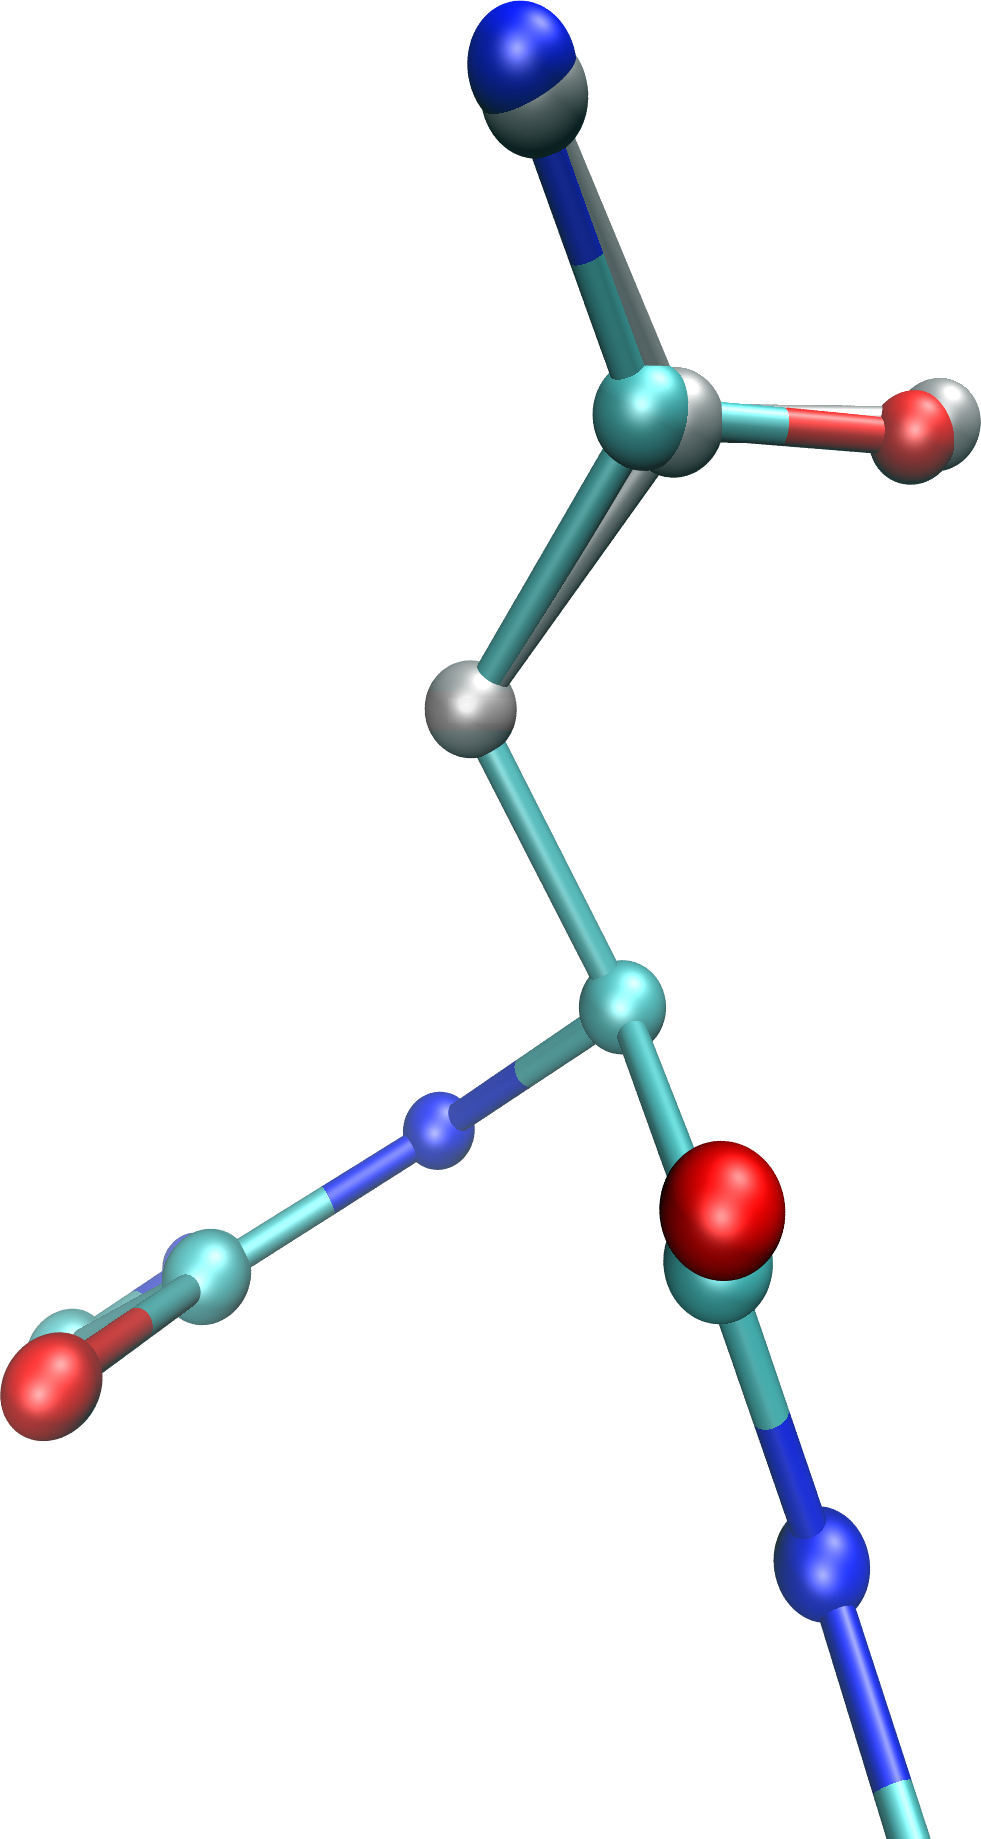
\includegraphics[width=0.65\textwidth,height=0.3\textheight,keepaspectratio]{figures/mutation_side_chain_images/1brs_chain_a_resid_58.png}
    \caption{Crystal (colored by element) and predicted (gray) side chain conformations for barnase, asparagine 58 of 1BRS.
    The predicted and crystal conformations are almost identical, differing by only 0.121 angstroms, or less than the resolution of the crystal structure.}
    \label{figure:computational_mutation_scanning/1brs_a_58}
\end{figure}

Figure \ref{figure:computational_mutation_scanning/1brs_a_73} shows a similar comparison for glutamic acid 73, which was one of the least successful predictions in this complex.
However, it would still be classified as a successful side chain prediction for many purposes, differing from the crystal structure by 0.993 angstroms.
\begin{figure}[h]
    \centering
    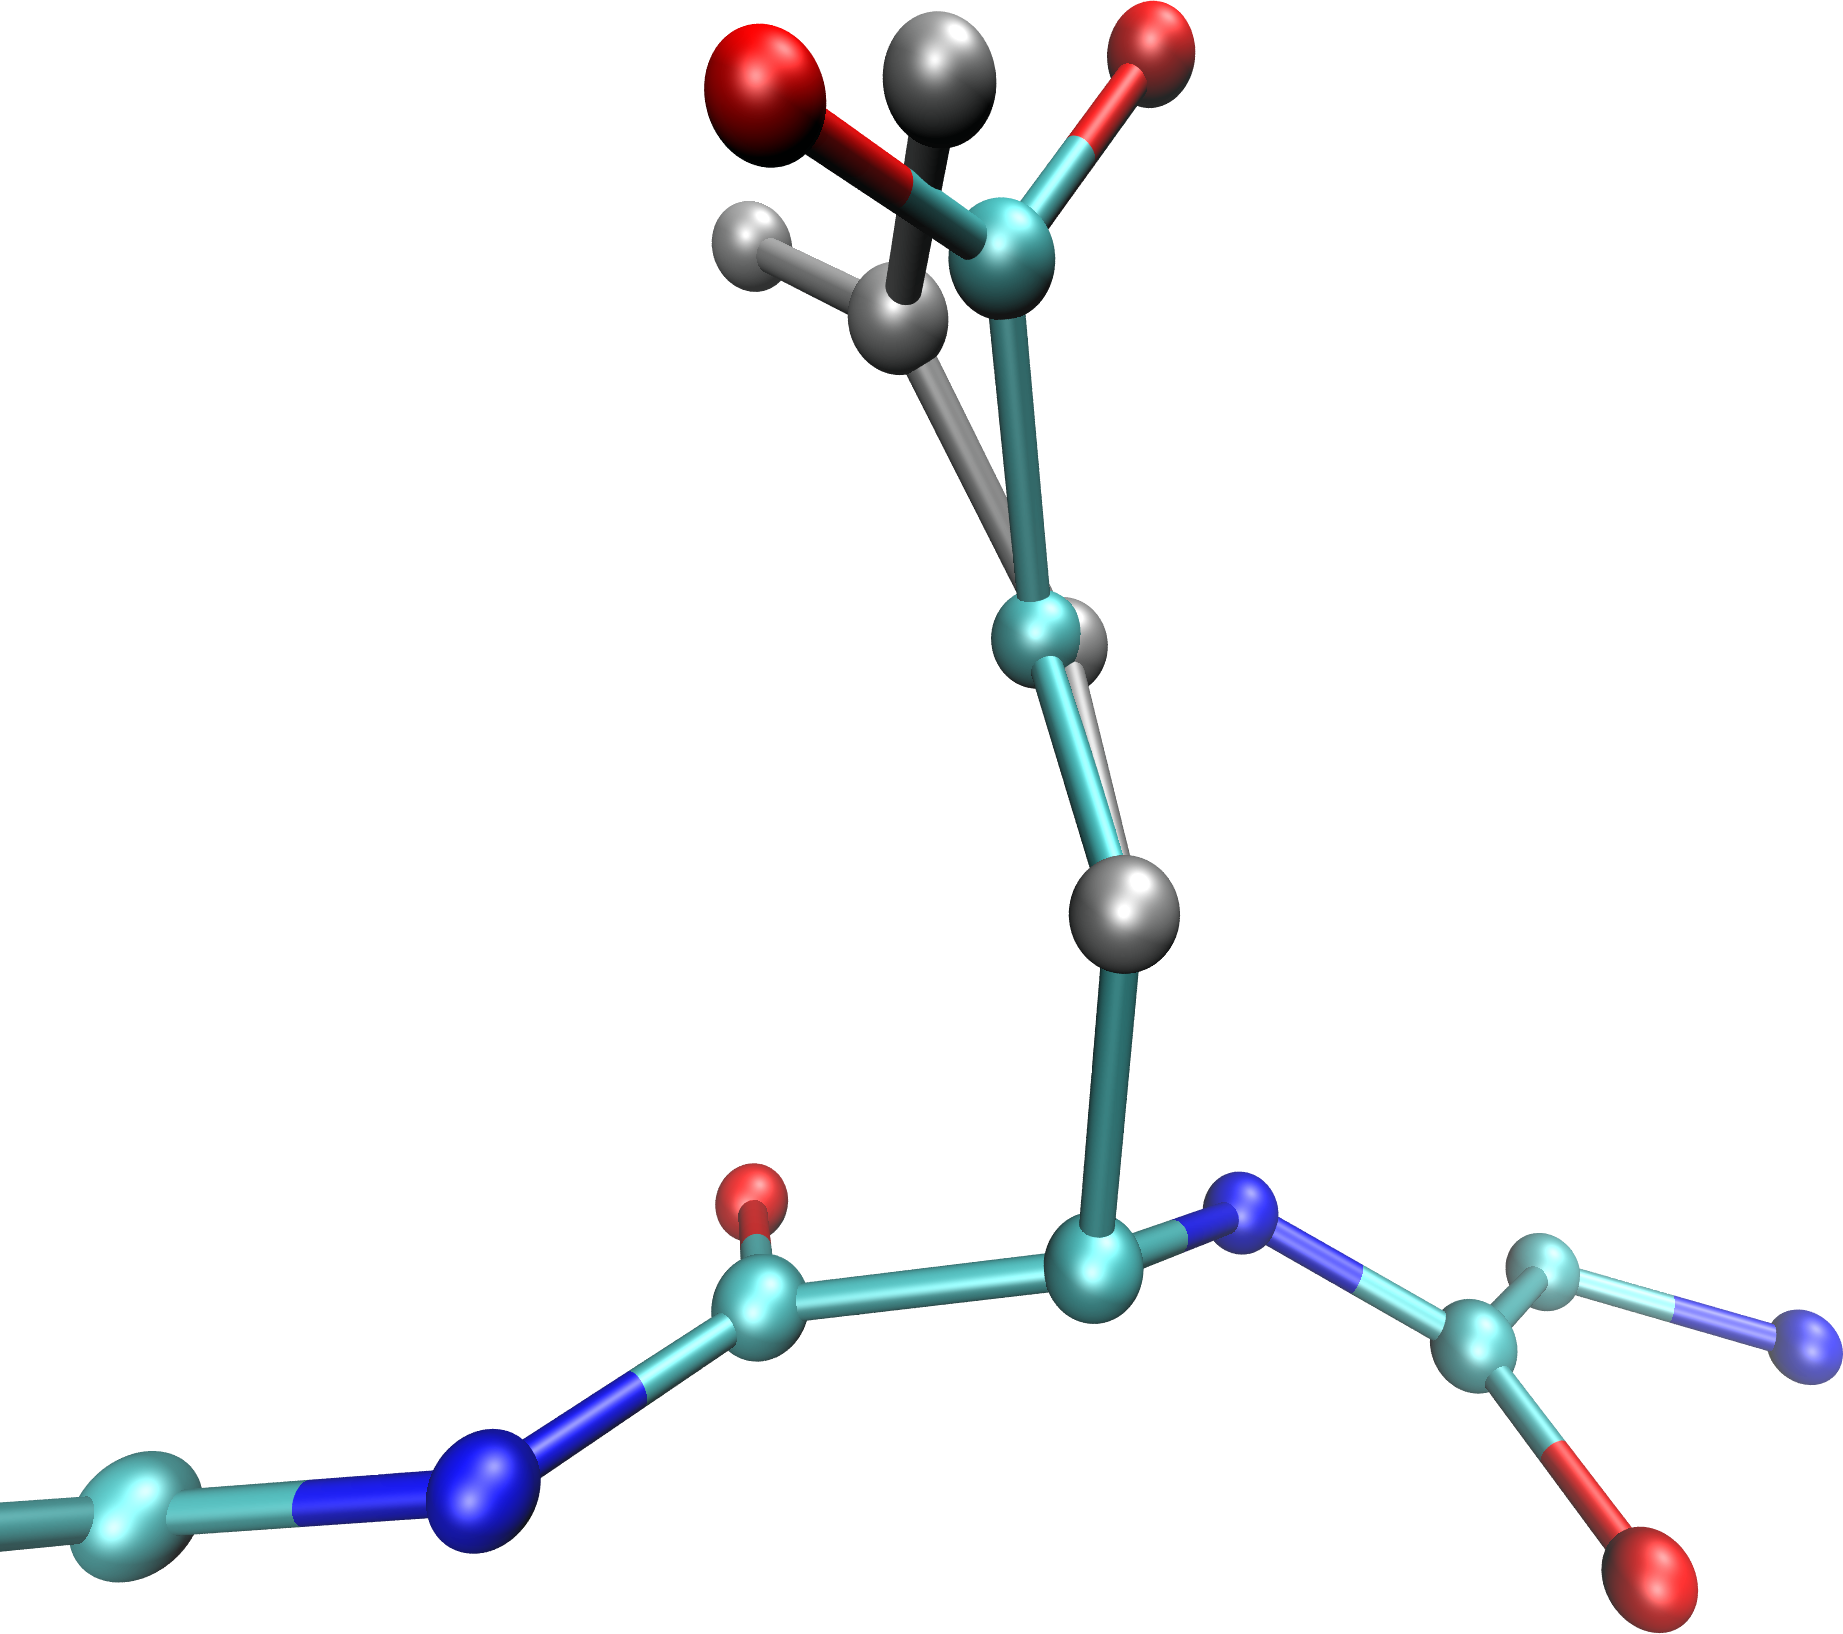
\includegraphics[width=0.65\textwidth,height=0.3\textheight,keepaspectratio]{figures/mutation_side_chain_images/1brs_chain_a_73.png}
    \caption{Crystal (colored by element) and predicted (gray) side chain conformations of glutamic acid 73 of barnase, chain A of PDBid 1BRS.
    The two conformations differ by 0.993 angstrom RMSD, which is generally considered a successful side chain prediction.}
    \label{figure:computational_mutation_scanning/1brs_a_73}
\end{figure}

%%%%%%%%%%%%%%%%%%%%%%%%%%%%%%%%%%%%%%%%%%%%%%%%%%%%%%%%%%%%%%%%%%%%%%%%%%%%%%%%%%%%%%%%%%%%%%%%%%%%
% 1BRSd
\FloatBarrier
\subsection{Barstar-Barnase Complex (Barstar Mutated)}
The second example makes use of the same complex, but it is the other partner of the complex, barstar, which is mutated.
The results here are similar to the previous case, in which figure \ref{figure:computational_mutation_scanning/1BRSd_ddg} shows that there is little correlation between computed and experimental \ddg, $R^{2}=0.21$.

\begin{figure}[h]
    \centering
    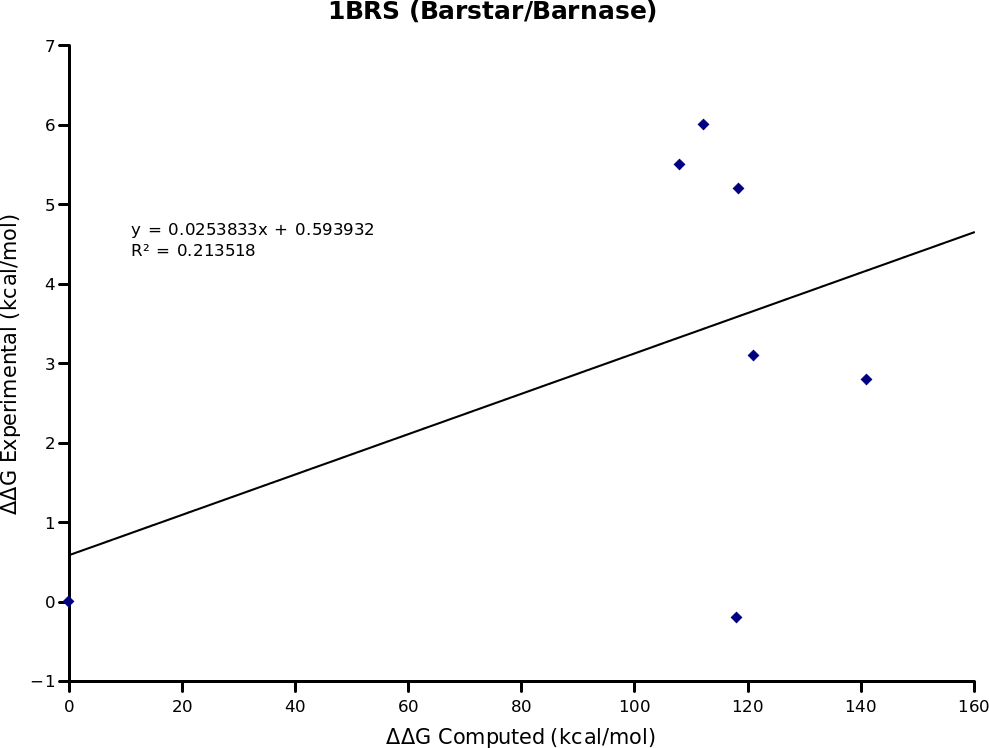
\includegraphics[width=0.65\textwidth]{figures/1brs_barstar_barnase.png}
    \caption{Computed versus experimental \ddg\ binding for 6 alanine mutations in the Barstar-Barnase binding pair.
    Crystal structure used for computations was 1BRS \protect\cite{buckle1994protein}.
    Specific amino acids mutated were residues 29, 35, 39, 42, 74, and 78, all of chain D.
    Experimental binding affinity taken from \protect\cite{thorn2001asedb}.}
    \label{figure:computational_mutation_scanning/1BRSd_ddg}
\end{figure}

Table \ref{table:1BRSd_results} shows the predicted and experimental \ddg\ binding for the barstar-barnase complex, depicted in figure \ref{figure:computational_mutation_scanning/1BRSd_ddg}.
\begin{table}[h]
\centering
\label{table:1brs_d_results}
\begin{tabular}{|c|c|c|}
\hline
Residue & \ddg\ calculated & \ddg\ experimental \\
\hline
native & 0 & 0 \\
29 & 121.07 & 3.1 \\
35 & 118.37 & 5.2 \\
39 & 118.09 & -0.2 \\
42 & 141.09 & 2.8 \\
74 & 107.92 & 5.5 \\
78 & 112.14 & 6 \\
\hline
\end{tabular}
\caption{Calculated and experimental \ddg\ for mutating given residues of barstar (chain D of structure 1BRS) to alanine.
Experimental values taken from \protect\cite{thorn2001asedb}.}
\end{table}

Table \ref{table:1BRSd_rmsd} shows the agreement of sampled side chain conformations with the native conformations.
Five of six side chains are predicted within 0.4 angstroms of their native conformation, maintaining all native contacts, and supporting the ability of the sampling method to explore sufficiently native-like conformations that the energy model is able to differentiate native-like from non-native like conformations.
\begin{table}[!h]
\centering
\begin{tabular}{|c|c|c|}
\hline
Residue & Amino Acid & RMSD \\
\hline
D:29 & TYR & 0.121 \\
D:35 & ASP & 0.098 \\
D:39 & ASP & 0.335 \\
D:42 & THR & 0.114 \\
D:76 & GLU & 0.397 \\
D:80 & GLU & 1.804 \\
\hline
\end{tabular}
\caption{RMSD of mutated side chains in barstar, in a barnase-barstar complex (chain D of PDBid 1BRS), during the mutation scanning experiments.}
\label{table:1BRSd_rmsd}
\end{table}

Figure \ref{figure:computational_mutation_scanning/1brs_all}  illustrates this in general for the protein-protein interface.

\begin{figure}[h]
\centering
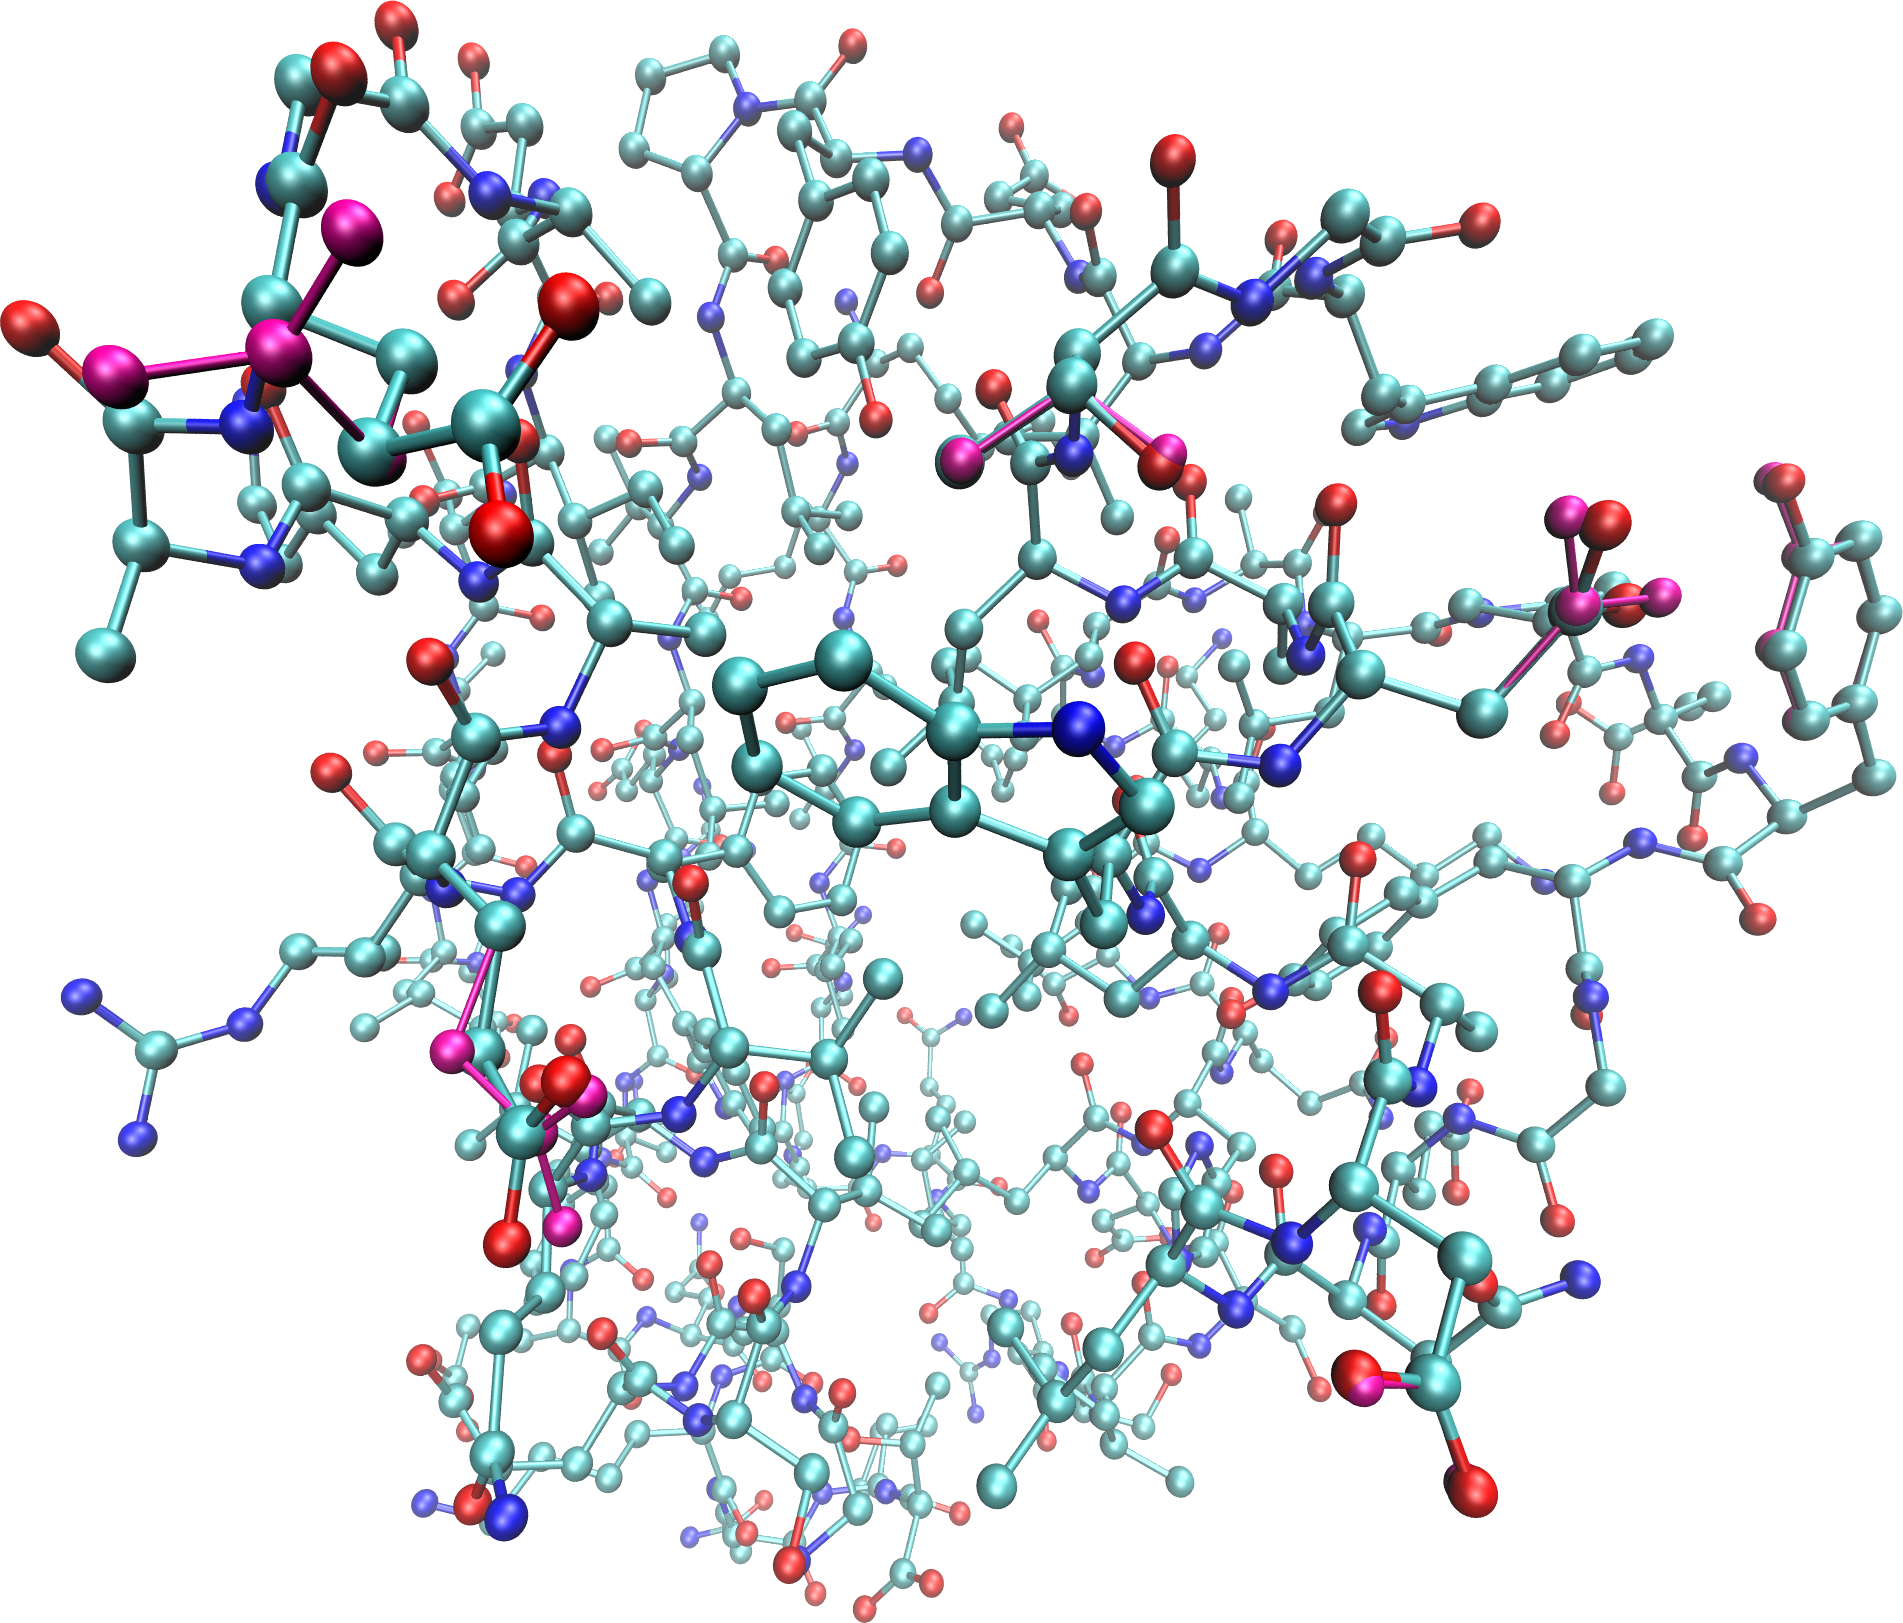
\includegraphics[width=0.65\textwidth,height=0.3\textheight,keepaspectratio]{figures/mutation_side_chain_images/1brs_all.png}
\caption{Distribution of 6 mutated residues (magenta) on the interface surface of barstar, 1BRS chain D.
Five of the six residues are less than 0.4 angstroms RMSD to the crystal structure.
The only exception is glutamic acid 80, shown in the upper left of this figure, and also figure \protect\ref{figure:computational_mutation_scanning/1brs_d_80}.}
\label{figure:computational_mutation_scanning/1brs_all}
\end{figure}

An example successful prediction is illustrated in \ref{figure:computational_mutation_scanning/1brs_d_35}.
The predicted conformation of this aspartic acid is less than 0.1 angstroms RMSD from its crystal conformation.
\begin{figure}[h]
    \centering
    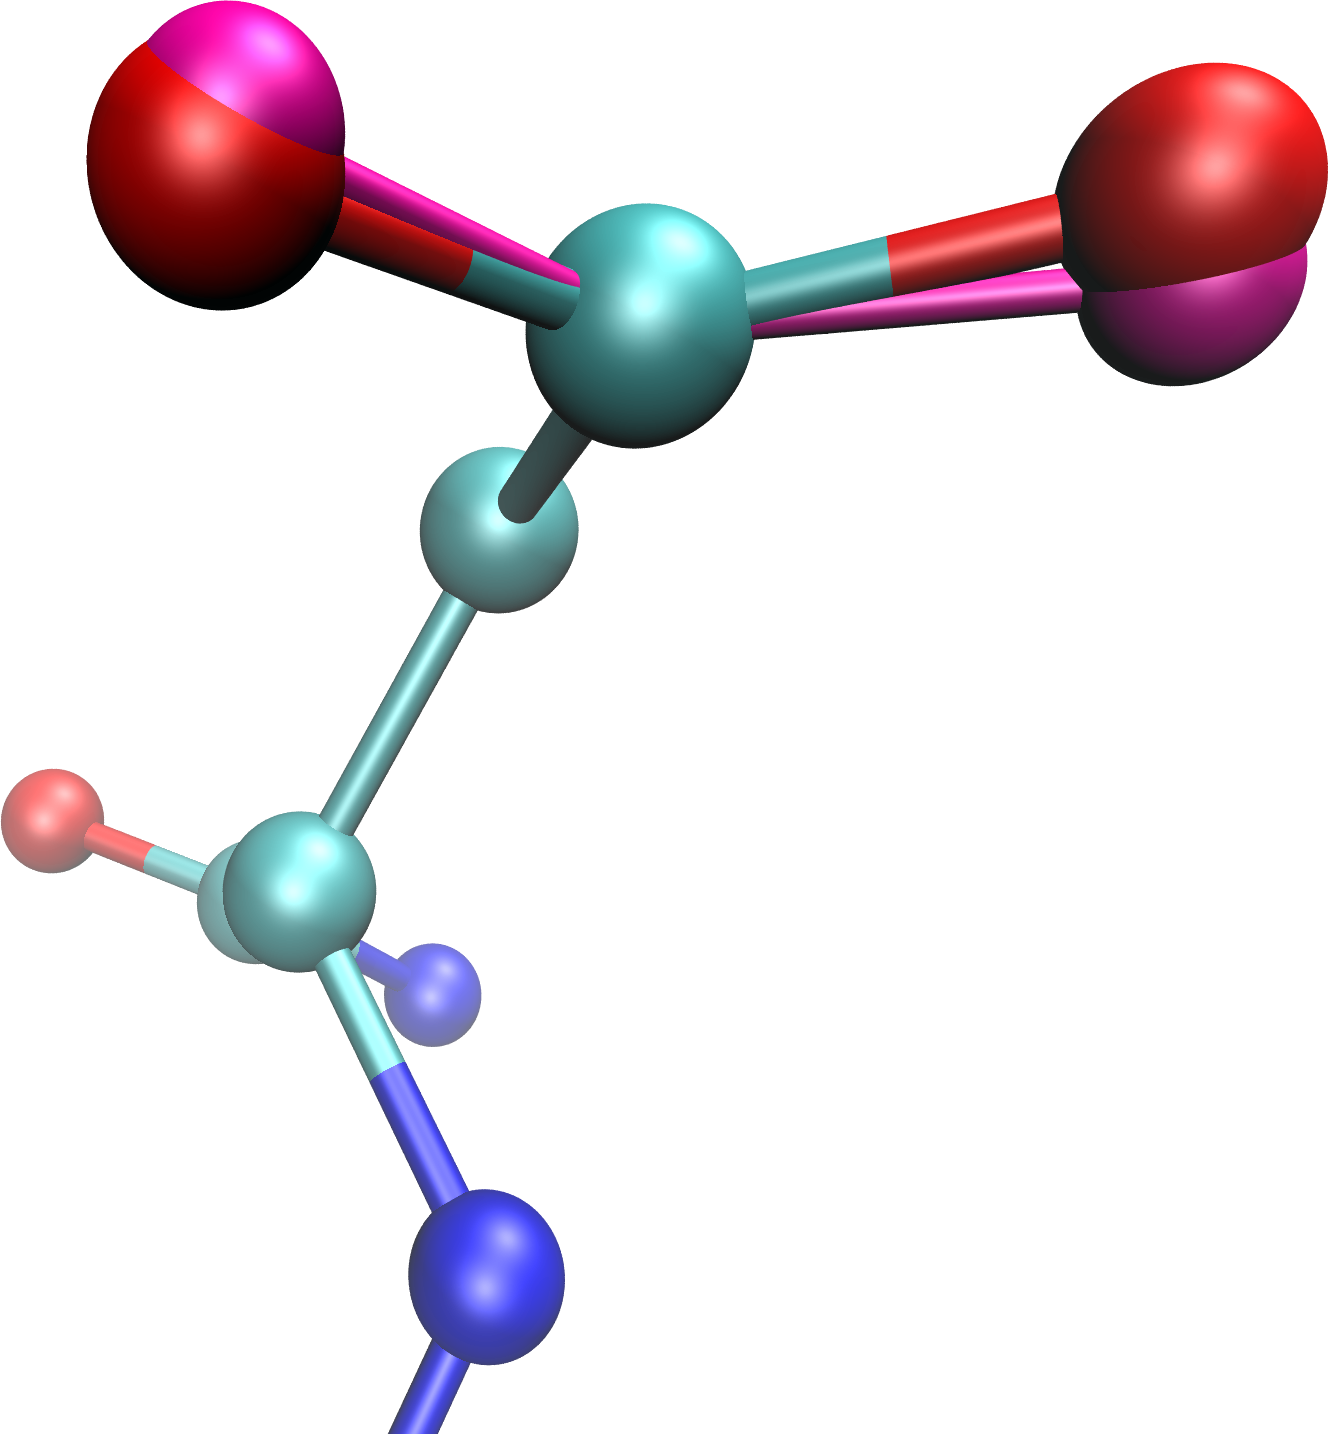
\includegraphics[width=0.65\textwidth,height=0.3\textheight,keepaspectratio]{figures/mutation_side_chain_images/1brs_chain_d_35.png}
    \caption{Crystal, colored by element, and predicted (magenta) side chain conformations for barstar, chain D of PDBid 1BRS.
    The distance to the crystal structure is only 0.098 angstroms, or nearly identical.}
    \label{figure:computational_mutation_scanning/1brs_d_35}
\end{figure}

The prediction which differs by the greatest amount from the crystal structure, Glu 80, is illustrated in \ref{figure:computational_mutation_scanning/1brs_d_80}.
While this predictions differs from the native by \textapprox 1.8 angstroms, this is still on the border of what is frequently considered a successful side chain prediction.
However, a prediction which differs from the native by this amount makes successfully predicting binding affinity difficult as the predicted conformation does not accurately recapitulate the contacts formed in the native complex.
\begin{figure}[h]
    \centering
    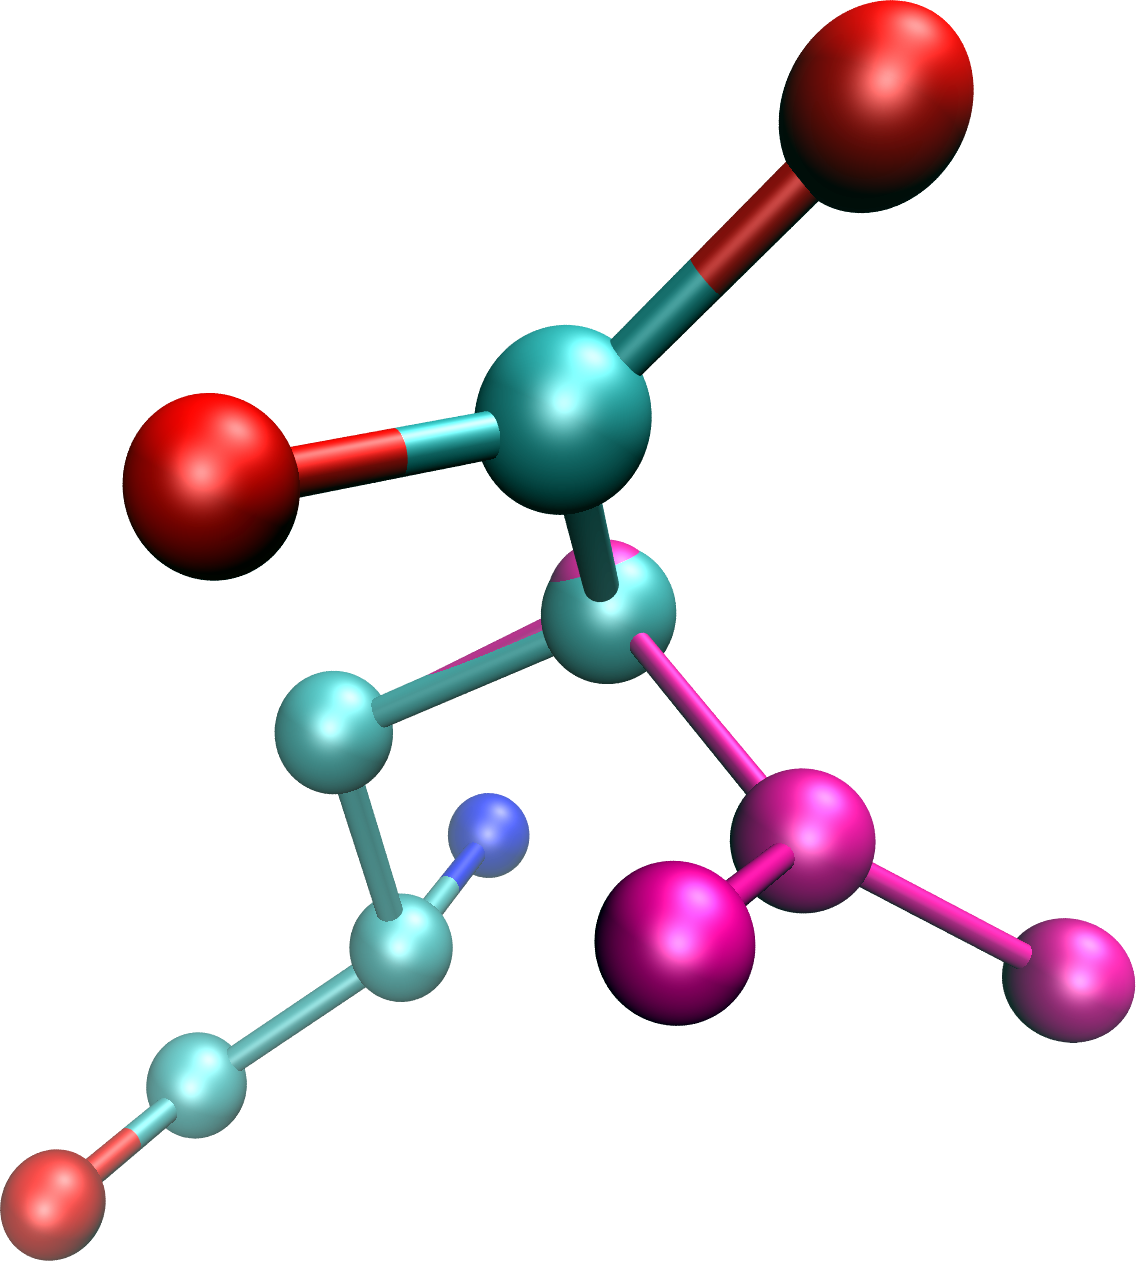
\includegraphics[width=0.65\textwidth,height=0.3\textheight,keepaspectratio]{figures/mutation_side_chain_images/1brs_chain_d_80.png}
    \caption{Glutamic acid 80 is the only residue on chain D, barstar, of the barnase-barstar complex which was not predicted within 0.4 angstroms of the crystal coordinates during the mutation scanning experiments.
    The difference between these two conformations is 1.804 angstroms, which while sometimes considered a ``successful'' prediction, is not sufficiently close to generate the same interactions, making it difficult to accurately predict binding affinities.}
    \label{figure:computational_mutation_scanning/1brs_d_80}
\end{figure}

%%%%%%%%%%%%%%%%%%%%%%%%%%%%%%%%%%%%%%%%%%%%%%%%%%%%%%%%%%%%%%%%%%%%%%%%%%%%%%%%%%%%%%%%%%%%%%%%%%%%
% 1DVF
\FloatBarrier
\subsection{Antibody anti-Antibody Complex}
The third example is an an antibody, anti-antibody complex.
The structure taken from PDBid 1DVF is of anti-hen-egg-white lysozyme antibody complexed with an antibody mimicking the hen egg white lysozyme \cite{braden1996crystal}.
As in the barnase-barstar complex examples there is no significant correlation between predicted and experimental \ddg\ (figure \ref{figure:computational_mutation_scanning/1DVF_ddg}).
The specific predicted and experimental values of \ddg\ are presented in table \ref{table:1BRSd_results}.

\begin{figure}[h]
    \centering
    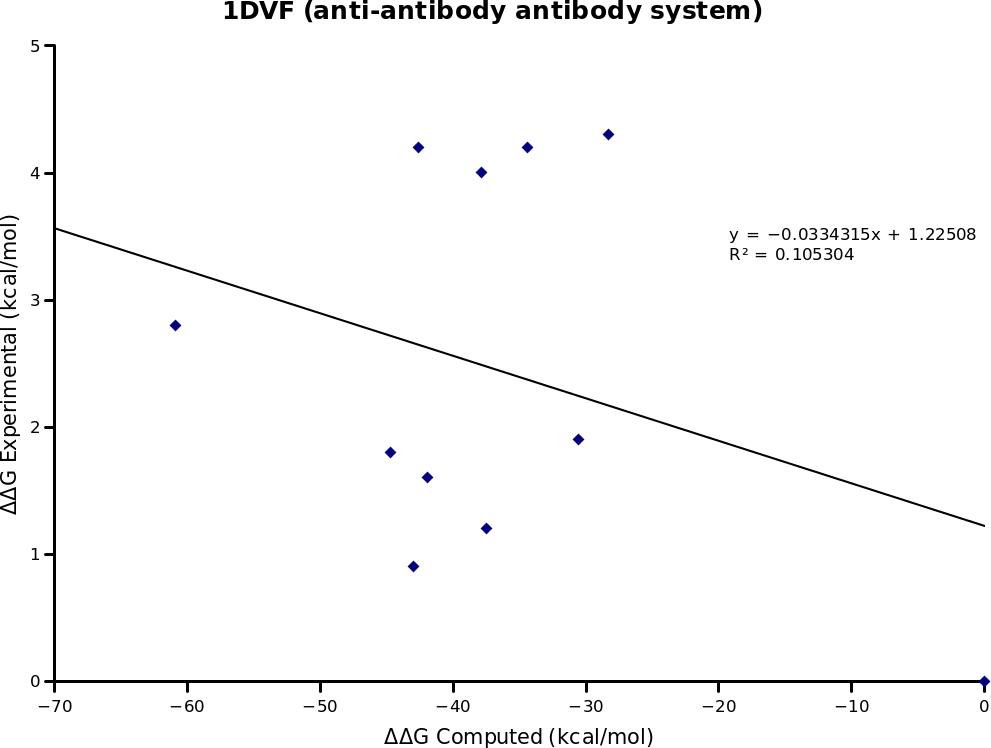
\includegraphics[width=0.65\textwidth]{figures/1dvf.png}
    \caption{Computed versus experimental \ddg\ binding for 10 alanine mutations in the anti-hen-egg-white lysozyme antibody (D1.3) anti-idiotopic antibody (E5.2) complex.
    Crystal structure used for computations was 1DVF \protect\cite{braden1996crystal}.
    Specific amino acids mutated were residues 30, 32, 52, 54, 56, 58, 98, 99, 100, and 101, all of chain A.
    Experimental binding affinity taken from \protect\cite{thorn2001asedb}.}
    \label{figure:computational_mutation_scanning/1DVF_ddg}
\end{figure}

\begin{table}[H]
\centering
\label{table:energy_timings}
\begin{tabular}{|c|c|c|}
\hline
Residue & \ddg\ calculated & \ddg\ experimental \\
\hline
native & 0 & 0 \\
30 & -42.93 & 0.9 \\
32 & -44.68 & 1.8 \\
52 & -42.6 & 4.2 \\
54 & -28.29 & 4.3 \\
56 & -37.5 & 1.2 \\
58 & -41.91 & 1.6 \\
98 & -34.38 & 4.2 \\
99 & -30.51 & 1.9 \\
100 & -60.9 & 2.8 \\
101 & -37.84 & 4 \\
\hline
\end{tabular}
\caption{}
\end{table}


Table \ref{table:1DVF_rmsd} shows the RMSD of side chains of 1DVF predicted during mutation scanning experiments.
The majority of side chains predicted were very close to the native conformation.
The most significant exception was aspartic acid 100, shown in figure \ref{figure:computational_mutation_scanning/1DVF_b_100}.
\begin{table}[!h]
\centering
\begin{tabular}{|c|c|c|}
\hline
Residue & Amino Acid & RMSD \\
\hline
B:30 & THR & 0.056 \\
B:32 & TYR & 0.412 \\
B:52 & TRP & 0.391 \\
B:54 & ASP & 0.442 \\
B:56 & ASN & 0.238 \\
B:58 & ASP & 0.159 \\
B:98 & GLU & 0.182 \\
B:99 & ARG & 1.137 \\
B:100 & ASP & 2.577 \\
B:101 & TYR & 0.340 \\
\hline
\end{tabular}
\caption{RMSD of mutated side chains in 1DVF, anti-hen-egg-white lysozyme antibody (D1.3) complexed with an anti-idiotopic antibody (E5.2), during the mutation scanning experiments.}
\label{table:1DVF_rmsd}
\end{table}


\begin{figure}[h]
    \centering
    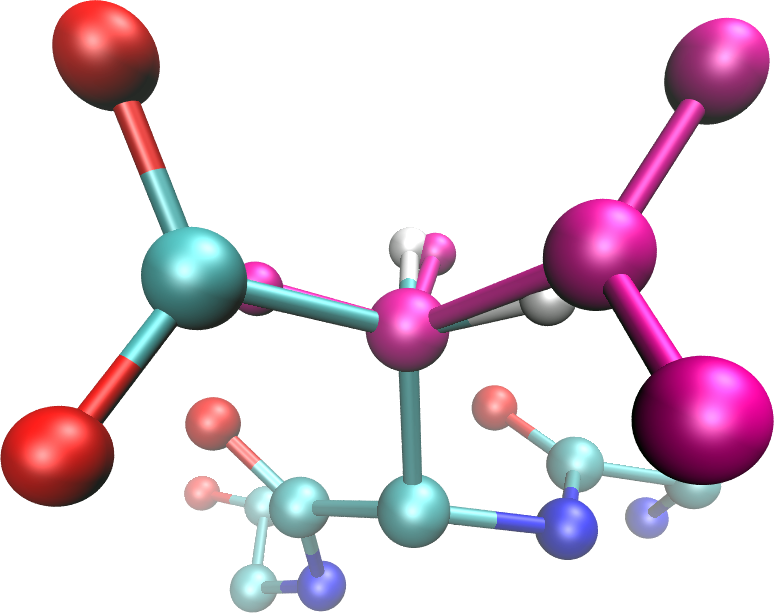
\includegraphics[width=0.5\textwidth,height=0.2\textheight,keepaspectratio]{figures/mutation_side_chain_images/1dvf_chain_b_100.png}
    \caption{An unsuccessful side chain prediction in the antibody antigen complex of PDBid 1DVF.  
    The predicted conformation of this aspartic acid, B:100, differs from the native state by 2.577 angstroms.}
    \label{figure:computational_mutation_scanning/1DVF_b_100}
\end{figure}

Two adjacent and successfully predicted side chains are, threonine 30 and tyrosine 32, with RMSDs of 0.056 and 0.412 angstroms respectively.
\begin{figure}[h]
    \centering
    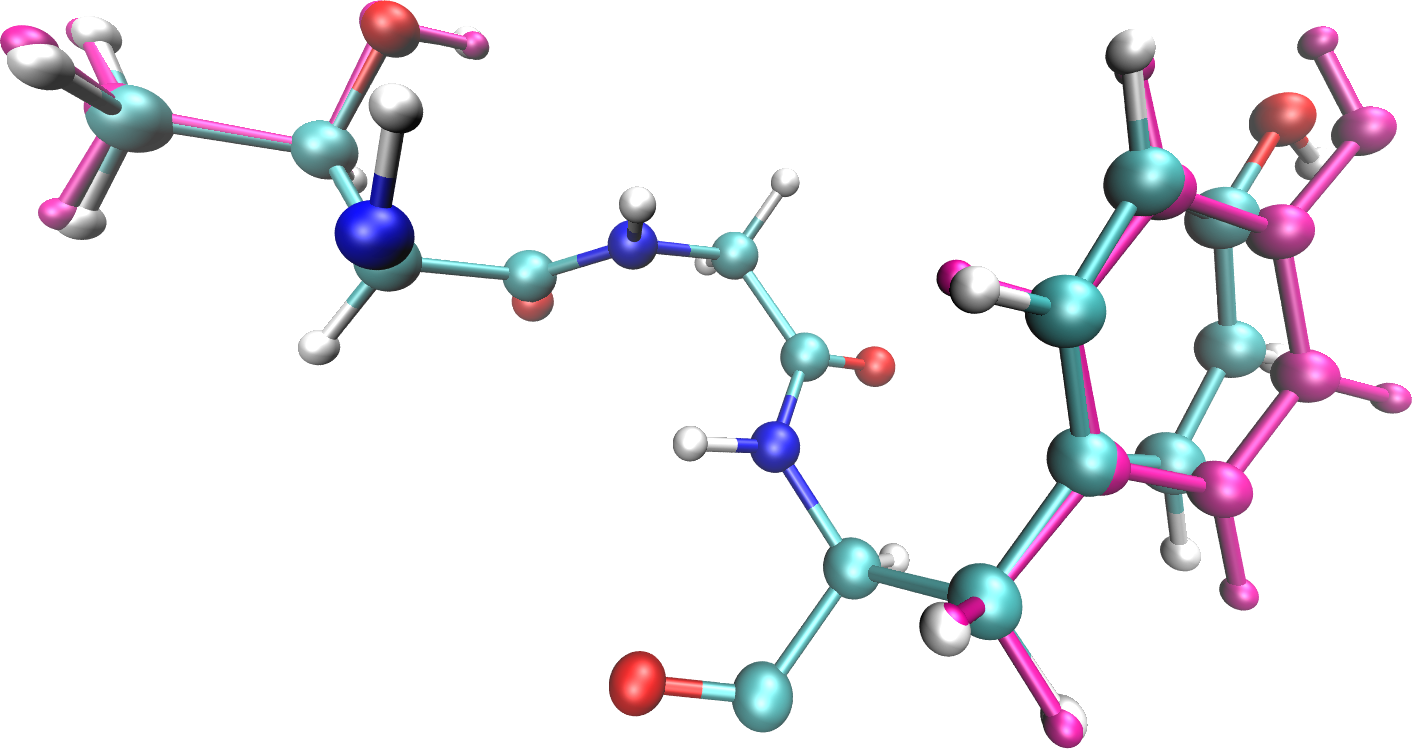
\includegraphics[width=0.65\textwidth,height=0.3\textheight,keepaspectratio]{figures/mutation_side_chain_images/1dvf_chain_b_30_and_32.png}
    \caption{Two neighboring successful predictions (magenta) in the same antibody antigen complex.
    Threonine 30, left, is predicted almost identically to the native structure, at 0.056 angstroms from the crystal coordinates.
    Tyrosine 32, right, is predicted at 0.412 angstroms RMSD.}
    \label{figure:computational_mutation_scanning/1DVF_B_30_and_32}
\end{figure}

%%%%%%%%%%%%%%%%%%%%%%%%%%%%%%%%%%%%%%%%%%%%%%%%%%%%%%%%%%%%%%%%%%%%%%%%%%%%%%%%%%%%%%%%%%%%%%%%%%%%
% 1FCC
\FloatBarrier
\subsection{Streptococcal Protein G fragment, IgG Antibody Complex.}
The final complex considered is another antibody antigen complex.
PDBid 1FCC depicts a fragment from streptococcal protein G in complex with an IgG antibody.
As in the previous cases there is little agreement between predicted and experimental \ddg\ binding, $R^{2}=0.40$, as shown in figure \ref{figure:computational_mutation_scanning/1FCC_ddg}.

\begin{figure}[h]
    \centering
    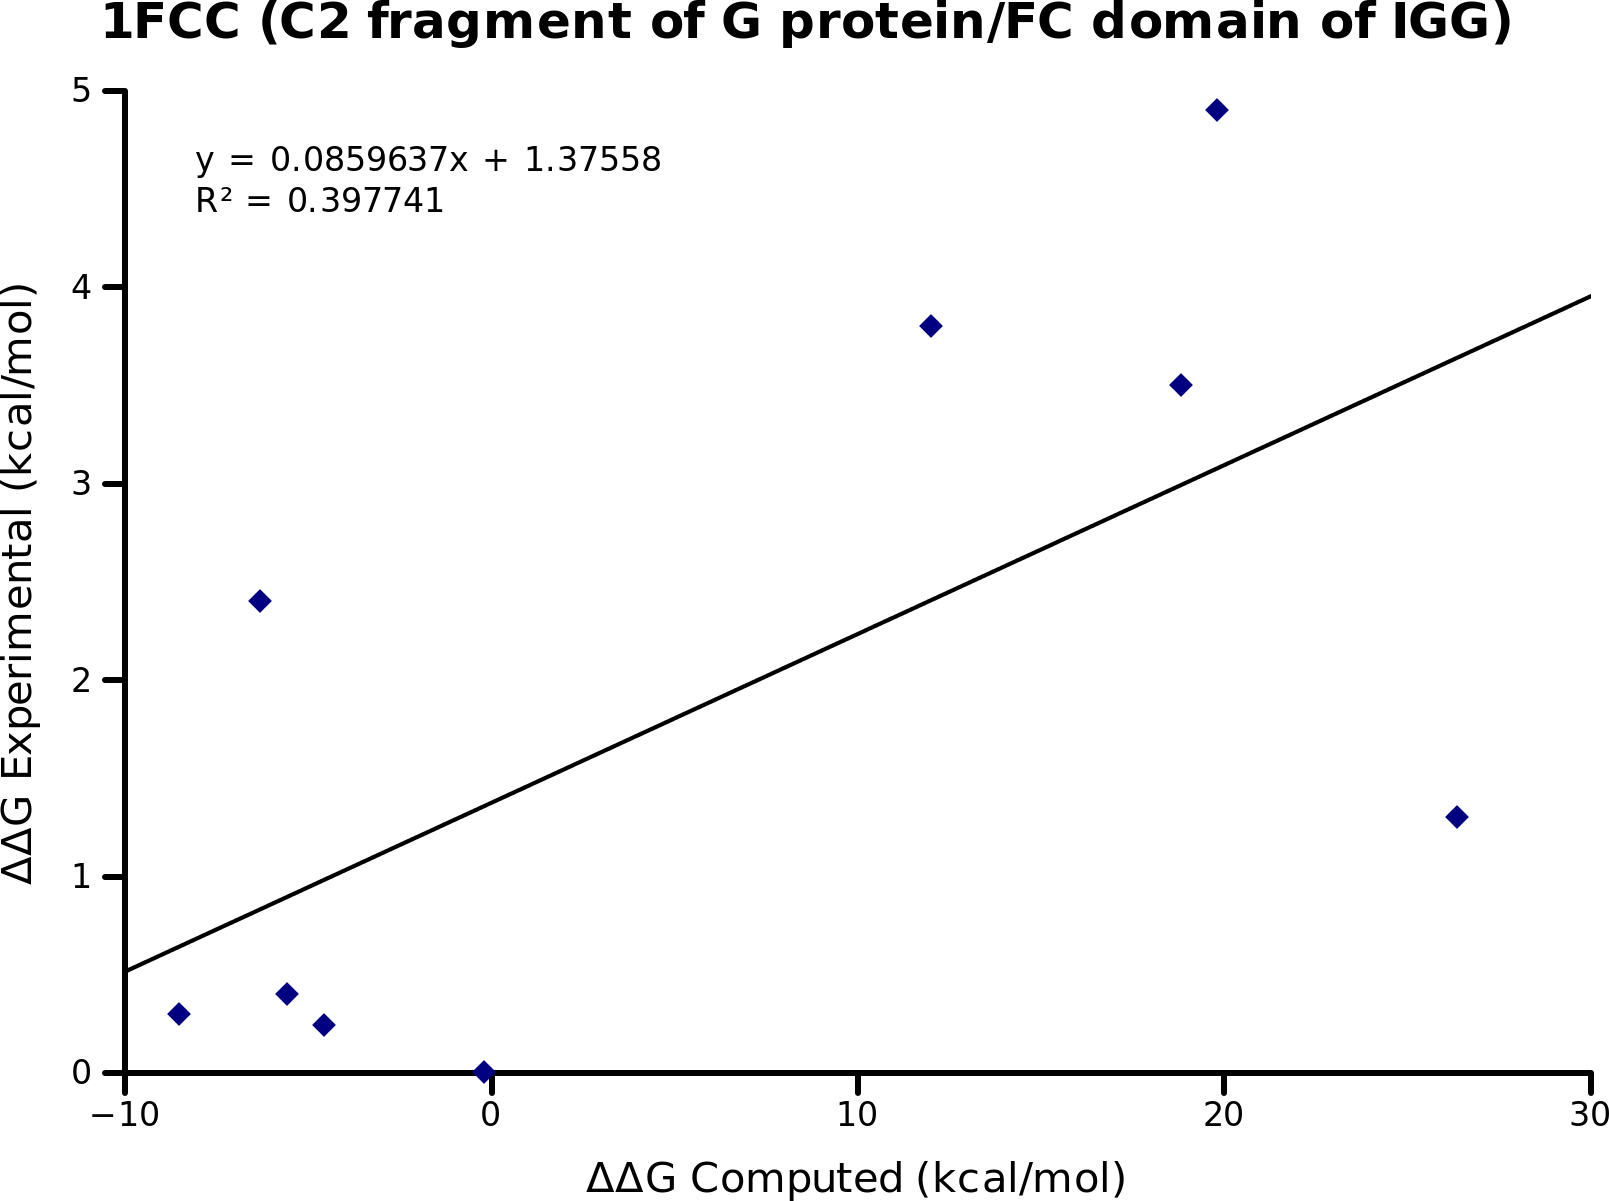
\includegraphics[width=0.65\textwidth]{figures/1fcc.png}
    \caption{Computed versus experimental \ddg\ binding for 8 alanine mutations in  binding pair.
    Crystal structure used for computations was 1FCC.
    Specific amino acids mutated were residues 25, 27, 28, 31, 35, 40, 42, and 43, all of chain A.
    Experimental binding affinity taken from \protect\cite{thorn2001asedb}.}
    \label{figure:computational_mutation_scanning/1FCC_ddg}
\end{figure}

\begin{table}[h]
\centering
\begin{tabular}{|c|c|c|}
\hline
Residue & \ddg\ calculated & \ddg\ experimental \\
\hline
native & -0.18 & 0 \\
25 & -4.55 & 0.24 \\
27 & 19.8 & 4.9 \\
28 & 26.37 & 1.3 \\
31 & 18.82 & 3.5 \\
35 & -6.31 & 2.4 \\
40 & -8.51 & 0.3 \\
42 & -5.56 & 0.4 \\
43 & 12.0 & 3.8 \\
\hline
\end{tabular}
\caption{Calculated and experimental \ddg\ for mutating given residues of Fc domain of human IgG (chain A of structure 1FCC) to alanine.
Experimental values taken from \protect\cite{thorn2001asedb}.}
\label{table:1FCC_results}
\end{table}


Table \ref{table:1FCC_rmsd} shows the RMSD of side chains of 1FCC predicted during mutation scanning experiments.
Seven of eight sampled side chains were predicted within 1.3 angstroms of native, and six of eight were within 0.6 angstroms of native.
As in the case of 1DVF the incorrect side chain prediction was a carboxylic acid, glutamic acid 42, where the predicted conformation differed from the crystal structure by almost 3 angstroms.
The most significant exception was aspartic acid 100, shown in figure \ref{figure:computational_mutation_scanning/1DVF_b_100}.
\begin{table}[!h]
\centering
\begin{tabular}{|c|c|c|}
\hline
Residue & Amino Acid & RMSD \\
\hline
C:25 & THR & 0.170 \\
C:27 & GLU & 0.403 \\
C:28 & LYS & 0.543 \\
C:31 & LYS & 0.594 \\
C:35 & ASN & 0.527 \\
C:40 & ASP & 1.292 \\
C:42 & GLU & 2.994 \\
C:43 & TRP & 0.371 \\
\hline
\end{tabular}
\caption{RMSD of mutated side chains in 1FCC, C2 fragment of streptococcal protein G in complex with the Fc domain of human IgG, during the mutation scanning experiments.}
\label{table:1FCC_rmsd}
\end{table}


\begin{figure}[h]
  \centering
  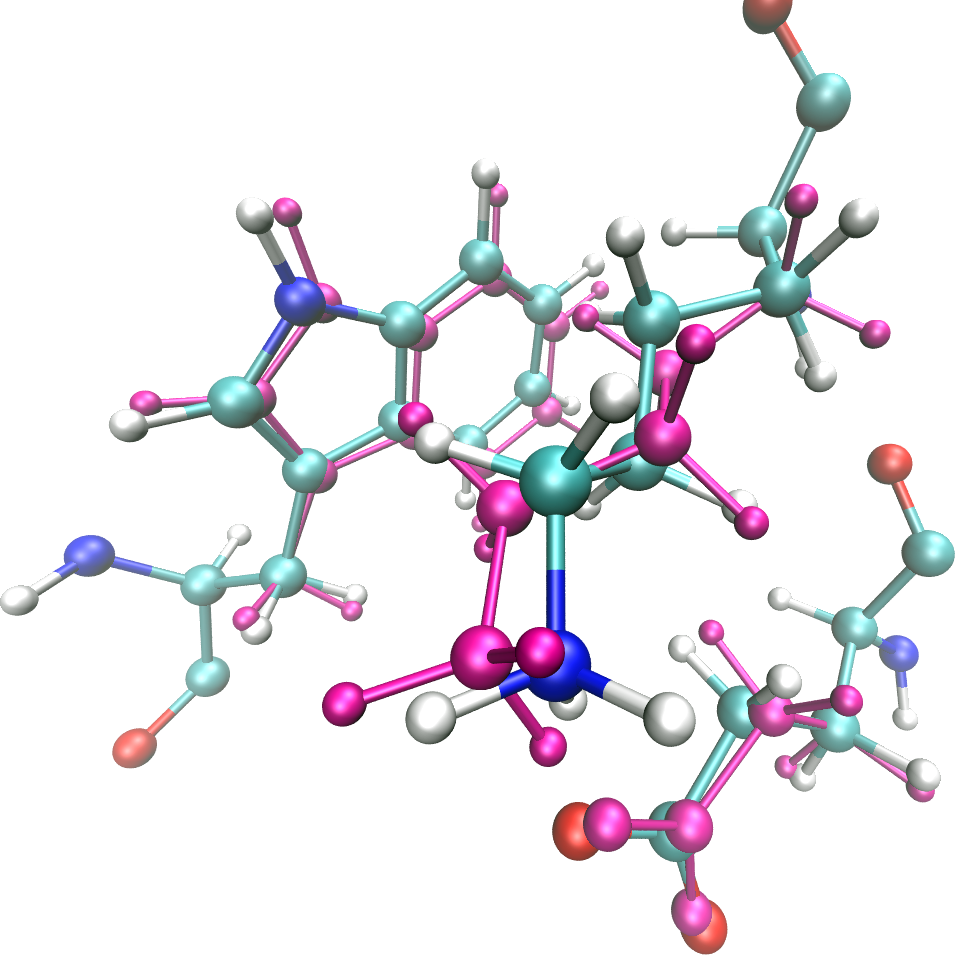
\includegraphics[width=0.65\textwidth,height=0.3\textheight,keepaspectratio]{figures/mutation_side_chain_images/1fcc_27_31_43.png}
  \caption{Three clustered hot spot residues in another antibody antigen complex, PDBid 1FCC, the C2 fragment of streptococcal protein G in complex with the Fc domain of human IgG.
The predicted conformations for glutamic acid 27, lysine 31 and tryptophan 43 are depicted in magenta, with side chain RMSD's of 0.403, 0.594 and 0.371, respectively.
These residues are shown in greater detail in other figures, glutamic acid 27 in figure \protect\ref{figure:computational_mutation_scanning/1FCC_27}, lysine 31 in figure \protect\ref{figure:computational_mutation_scanning/1FCC_31}, and tryptophan 43 in figure \protect\ref{figure:computational_mutation_scanning/1FCC_43}.}
  \label{figure:computational_mutation_scanning/1FCC_27_31_43}
\end{figure}

This side chain is in close proximity to a number of other hot spot residues on the protein-protein interface and is shown in context in figure \protect\ref{figure:computational_mutation_scanning/1FCC_27_31_43}.
\begin{figure}[h]
  \centering
  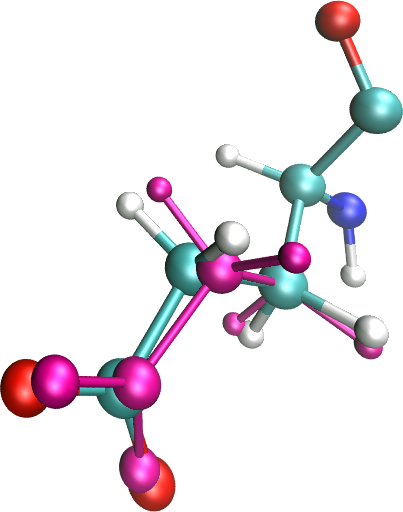
\includegraphics[width=0.65\textwidth,height=0.3\textheight,keepaspectratio]{figures/mutation_side_chain_images/1fcc_27.png}
  \caption{Predicted (magenta) and crystal conformations (colored by element) for glutamic acid 27.
The side chain RMSD of this prediction is 0.403 angstroms.}
  \label{figure:computational_mutation_scanning/1FCC_27}
\end{figure}

\begin{figure}[h]
  \centering
  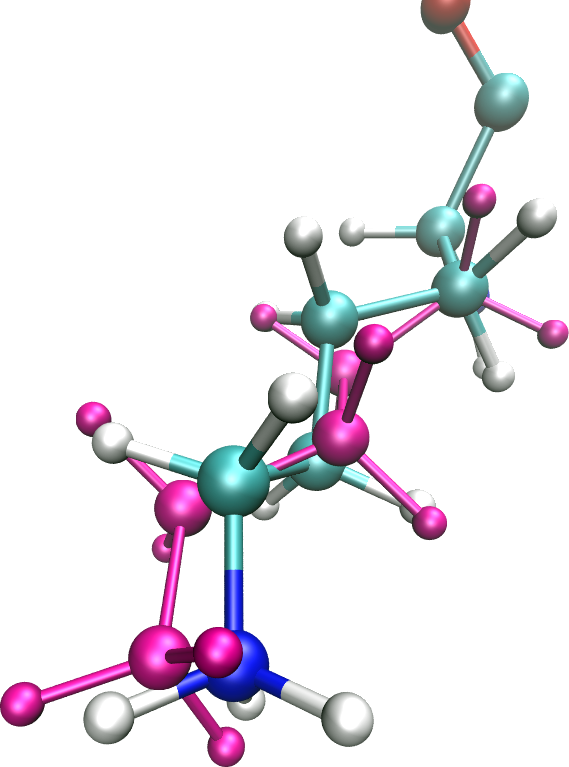
\includegraphics[width=0.65\textwidth,height=0.3\textheight,keepaspectratio]{figures/mutation_side_chain_images/1fcc_31.png}
  \caption{The predicted side chain conformation during the course of mutation scanning experiments (magenta) compared to the native conformation (colored by element) for lysine 31.
The RMSD of this prediction is 0.594 angstroms.}
  \label{figure:computational_mutation_scanning/1FCC_31}
\end{figure}

\begin{figure}[h]
  \centering
  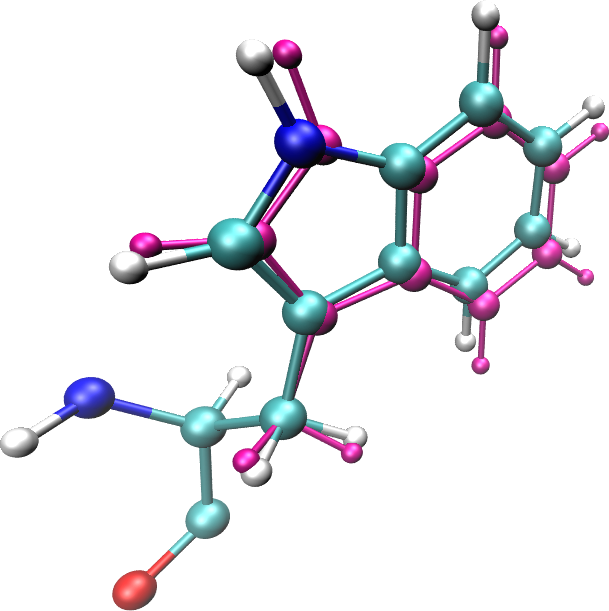
\includegraphics[width=0.65\textwidth,height=0.3\textheight,keepaspectratio]{figures/mutation_side_chain_images/1fcc_43.png}
  \caption{Native (colored by element) and predicted (magenta) side chain conformation for tryptophan 43 of 1FCC.
The root mean square distance of the predicted conformation to the native is 0.371 angstroms.
The effect of the local protein structure on the conformation of this residue is examined in figure \protect\ref{figure:1fcc_43_pocket}.}
  \label{figure:computational_mutation_scanning/1FCC_43}
\end{figure}

Tryptophan 43 is interesting in that despite being critical to protein-protein binding it is largely buried in a pocket defined by the neighboring protein structure.
This interaction is examined in figure \protect\ref{figure:1fcc_43_pocket}.
\begin{figure}[h]
    \centering
    \begin{subfigure}[b]{0.3\textwidth}
        \centering
        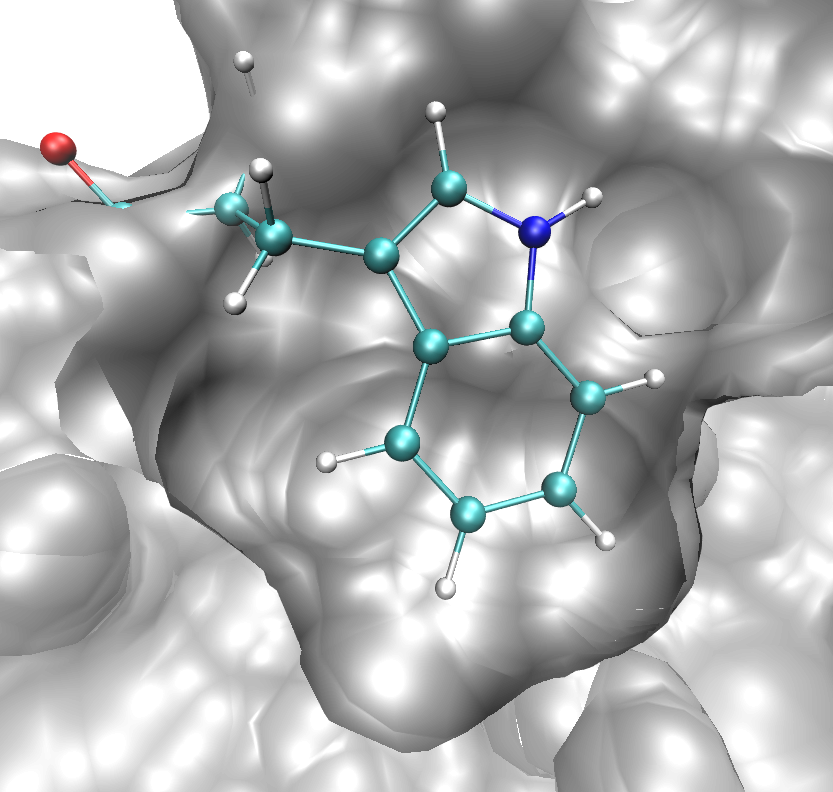
\includegraphics[width=\textwidth,height=\textheight,keepaspectratio]{figures/mutation_side_chain_images/in_pocket_out_of_plane.png}
        \caption{}
        \label{figure:mutation_side_chain_images/in_pocket_out_of_plane}
    \end{subfigure}
    \hspace{0.1\textwidth}
    \begin{subfigure}[b]{0.3\textwidth}
        \centering
        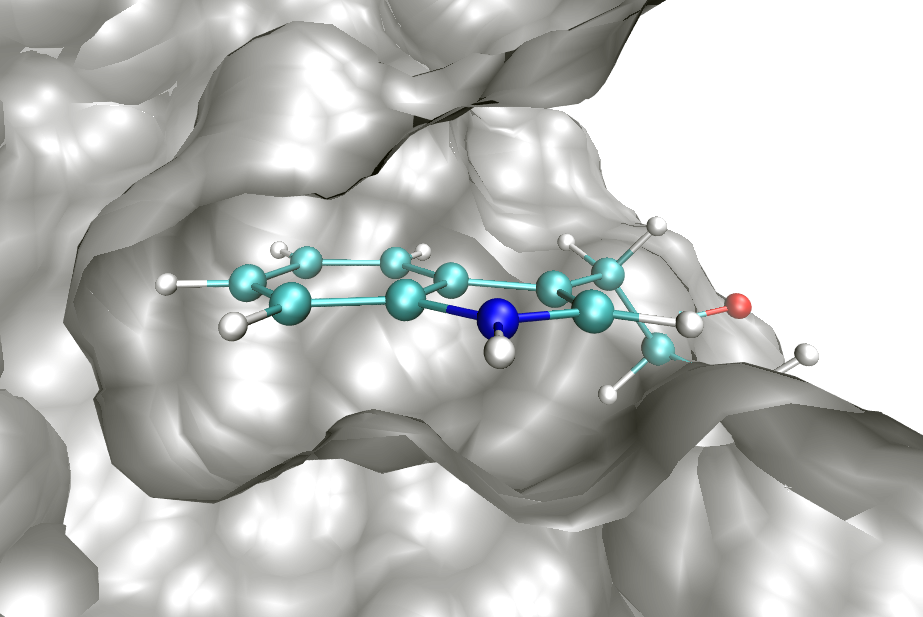
\includegraphics[width=\textwidth,height=\textheight,keepaspectratio]{figures/mutation_side_chain_images/in_pocket_in_plane.png}
        \caption{}
        \label{figure:mutation_side_chain_images/in_pocket_in_plane.png}
    \end{subfigure}
    \caption{The pocket of tryptophan 43 of 1FCC, shown in two orthogonal orientations \label{figure:mutation_side_chain_images/in_pocket_out_of_plane} and \label{figure:mutation_side_chain_images/in_pocket_in_plane.png}.
Because of conformation of the neighboring protein structure, this residue has very little conformational freedom, and any prediction which successfully locates the side chain in the pocket will be reasonably close to the native state.
The conformation predicted in these experiments was very similar, 0.371 angstroms, and is depicted superimposed with the native in figure \protect\ref{figure:computational_mutation_scanning/1FCC_43}.}
    \label{figure:1fcc_43_pocket}
\end{figure}


